\section{Confirm Service Activity Solutions}
\label{confirm-service-activity}
As discussed previously, for confirm service activity we need secure solutions that allow an Ursula to prove that she has served a given number of distinct re-encryption requests within a given period. In particular, for every round an Ursula will need to produce a proof attesting to the statement ``Ursula has served $\omega$ distinct re-encryption requests correctly," for some positive integer $\omega$. In this section, we present three solutions to achieve this goal, which we refer to as zero knowledge proof-based (ZKP-based), committee-attestation, and commit/challenge/open-based. These solutions differ in their security assumptions, guarantees, proof technique, and efficiency. In what follows, we provide the design details of each of them.


\subsection{ZKP-based Scheme}
In this solution, we utilize the fact that in the NuCypher network each Ursula already produces a ZKP attesting to the correctness of each re-encryption request she performs to be checked by Bob~\cite{umbral2018}. Such proofs can be aggregated into a single proof attesting to the statement outlined above. This accumulation can be done using two approaches: by using generic techniques like proof carrying data (PCD)~\cite{chiesa2010proof} or incrementally verifiable computation (IVC)~\cite{valiant08}, or by using a ZKP system for arithmetic circuits. 


For the generic PCD/IVC approach, we have only one prover or computation party, namely, Ursula. For each round, Ursula starts with input $x_1$, which is a signed and fresh re-encryption request from Bob. It answers this request with a ciphertext fragment $cFrag_{x_1}$ and produces a correctness proof $\pi_1$ as defined in the Umbral scheme~\cite{umbral2018}. Then, when the next request $x_2$ arrives, which is the input for the next step in the computation, Ursula answers this request as before and produces $cFrag_{x_2}$ and a correctness proof $\pi_2$, then it uses $(x_2, cFrag_{x_2}, \pi_2)$ and the previous proof $\pi_1$ to produce $\hat{\pi}_2$. $\hat{\pi}_2$ does not only attest to the correctness of $cFrag_{x_2}$, but also attests to the fact that Ursula has served two valid distinct requests until now. The same process is repeated until all requests served in a round are covered. At the end, Ursula produces a single proof $\hat{\pi}_{\omega}$ along with the number of served requests $\omega$ as the final proof. Figure~\ref{pcd-based-sol} depicts this process pictorially.


\begin{figure}[h!]
\centerline{
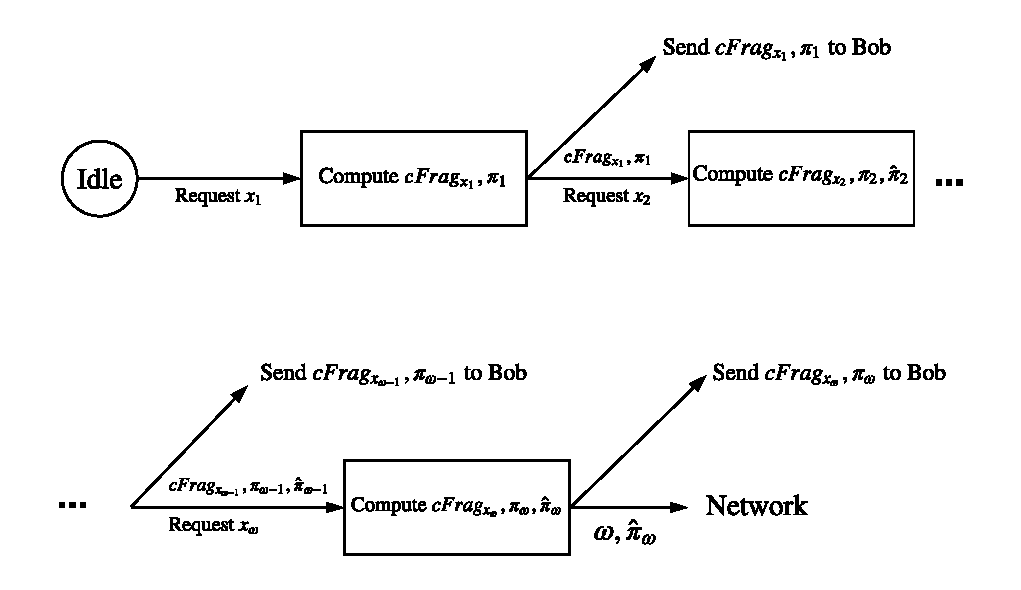
\includegraphics[height= 2.5in, width = 1.0\columnwidth]{figures/pcd-based-sol.pdf}}
\caption{PCD-based solution diagram. Ursula starts a round in the idle state. When the first request arrives, Ursula responds to the request and starts composing the proofs as new requests arrive. At the end of the round, Ursula informs the network (i.e., verifier) of the number of served requests and a single proof attesting to her claim. }
\label{pcd-based-sol}
\end{figure}


An alternative, possibly more efficient approach, is to view the statement ``Ursula has served $\omega$ distinct re-encryption requests correctly" as an instance of the arithmetic circuit satisfiability problem and utilize a highly efficient ZKP system, e.g., Bulletproofs~\cite{bunz18}, to prove its correctness in zero knowledge. That is, build a circuit that takes the set of correctness proofs of the served requests as well as their number $\omega$ as inputs, and then output 1 if number of correct distinct proofs equals to $\omega$. Then, invoke a circuit parser~\cite{bunz18} to convert the circuit into the Bulletproof format, which allow the prover, Ursula in this case, to produce a single proof. 


In both cases, Ursula submits a single proof to the service policy contract. Once the proof is verified, the contract disperses the service fee (in proportion to $\omega$) from Alice's locked Ether to Ursula's account.


\subsection{Committee-Attestation Scheme}
This solution shares a similar theme to confirm availability solution discussed previously. It relies on electing a committee for each round that will endorse Ursula's claim of serving $\omega$ distinct and valid re-encryption requests in a given round. The endorsement is done by employing CoSi (see Section~\ref{cosi}) to permit the committee to collectively sign the statement ``Ursula has served $\omega$ distinct re-encryption requests correctly."  


In detail, for each round, a committee of Ursulas (and possibly outsider verifiers) is elected to attest for the work load an Ursula served. At the end of a round, each working Ursula establishes a record of all the requests she served along with their individual correctness proofs and the ciphertext fragments she computed. Then, she initiates the CoSi protocol to sign the workload statement above, denoted as $m$, while replacing $\omega$ with the actual number of served requests in the round. Ursula sends $m$ along with the full service record to each member of the committee, which in turn verfiies the correctness of the report as follows: 

\begin{enumerate}
\item Check that each request is distinct by checking the sequence number/timestamp of the request.

\item Check that each request is valid by verifying Bob's signature over the request. (Here the policy will contain Bob's public key to allow the committee to use the right verification key.)

\item Verify the ZKP correctness proof of each $cFrag$ as in the Umbral scheme.

\item Check that the value of $\omega$ inside $m$ agrees with the record.
\end{enumerate}


If everything is fine, each member of the committee and the working Ursula finalize the CoSi signing protocol and produce one signature over $m$. At the end, the working Ursula publishes $m$ and the collective signature to the network, or the service policy contracts, which in turn verifies correctness as described in Section~\ref{cosi}.


\paragraph{\bf On the committee election.} 
For each round some reasonable number of Ursulas will be elected by using a similar technique to the ones described in Section~\ref{confirm-availability}, i.e., using the hash iterative process. The selection may also take into account the presence and size of each Ursula's stake, to avoid an attacker spinning up enormous numbers of Ursulas in order to increase the chance of them controlling the entire committee.


The above scheme works under the assumption that at least one Ursula in the elected committee is honest, which pertains to an assumption on the least number of honest Ursulas in the network. If the latter assumption is under threat, one mitigating approach is to increase the committee size. Another approach is to have a changing set of external verifiers, like trusted partners, as part of the elected committee. As long as there is one honest party in the committee, signing fraudulent records will not succeed since this honest party will not agree to do that.


\paragraph{\bf On the public verifiability of the signed records.} 
Having a valid collective signature from a committee (that has at least one honest member) suffices for the correctness of the signed statement. However, it could be better to keep the records that produced the message $m$ available for a while so that any party can verify them (the verifying parties could maintain such a public record for a given period after which the logs can be discarded). We can resort to this option just at the beginning to convince the participants of the trustworthiness of the committee or the validity of the assumption that at least one Ursula in the elected committee is honest. 


\paragraph{\bf On compensating the committee.} 
Similar to confirm availability, we need a mechanism to ensure that the elected committee is responsive and willing to handle the endorsement work. Ideally, this can be pictured as a collaborative work, the committee does the work so that others will do the same when the committee members want their workload to be signed. Alternatively, and as mentioned before, the committee can be paid for their work, either by Alice as part of her policy, or by the working Ursulas themselves since they are requesting this endorsement service (however, the latter may complicate the system operation).


\subsection{Commit/Challenge/Open-based Scheme}
This solution is inspired from the Merkle tree-based ZKP system proposed in~\cite{dottling19}. Ursula keeps track of the requests coming from Bob(s) during a time round and assign each of them a unique sequence number. That is, Ursula replies with $cFrag$ and the correctness proof. At the end of the round, Ursula constructs a Merkle tree of all requests, where the requests (and their replies/correctness proofs) are the leaves of the tree ordered by their sequence numbers (recall that we require Bob to include a sequence number in his request to ensure freshness). Ursula signs the root of the tree, denoted as $root$ to produce a signature $\sigma_{root}$


To prove correctness of the claimed work amount, Ursula will be challenged to open some leaves in the Merkle tree. She uses the $root$ as a random beacon to be fed into an iterative hash process to select $n$ leaf nodes at random to open them (i.e., these are the challenges). Ursula provides the challenge leaf nodes along with their membership paths in the tree, along with $(\omega, root, \sigma_{root})$, either to a sidechain (which is maintained by round-elected committee) or to the policy contract to verify. 


The verification process involves verifying Ursula's signature on the $root$, verifying the freshness and correctness of the request in each opened leaf, and verifying the membership path of each of these leaves. If everything is fine, Ursula will be paid for serving the claimed $\omega$ request.


It should be noted that the security provided here is statistical, driven by the value of $n$, in the sense that we need to bound the probability by which an Ursula can cheat, such as replicating requests in the tree and adding fabricated ones to increase $\omega$. 